
\section{Goals}\label{goals}

Modern mobile devices are equipped with various complex sensors --
accelerometers, location, video, audio, temperature, altitude, etc. Not
all of them provide scientific-grade precision or update frequency.
However these disadvantage are often compensated by ubiquity and
availability of such devices, allowing unprecedented deployment scale
for scientific experiments. We aim to create a piece of message-oriented
middleware which allows data to be gained from mobile devices without
the data recipient having to build a server architecture.

\section{Design}\label{design}

\subsection{Key protocols}\label{key-protocols}

As described in the brief, the sensor data producer is deployed on a
mobile device. This dictated a number of constraints that had to be
considered while developing the system; First, the technologies used to
develop the producer had to be easy to deploy on a mobile device. In
recent years, it has become increasingly popular to develop mobile web
apps -- applications that use the device's web browser as the execution
environment. Such applications have an advantage of being easy to
distribute and deploy on various platforms. HTML5 and Javascript, used
to develop web apps, provide rich APIs for accessing sensor data --
accelerometers, audio, video, etc. Thus, the project aimed to utilise
technologies that are supported by browsers of modern mobile platforms.

\subsubsection{WebSockets and WAMP}\label{websockets-and-wamp}

WebSockets is a protocol for full-duplex (two-way) communication through
TCP, meaning various aspects of reliability and robustness are taken
care of by the transport protocol (e.g.~in-order guaranteed messages).
Additionally, compared to regular HTTP requests, WebSockets have a low
header overhead (2 bytes compared to kilobytes in HTTP). Two-way
communication and low overhead (thus, decreased latency and bandwidth
usage) are advantageous for a data streaming platform.

WebSockets are supported by most modern desktop and mobile browsers
(through Javascript APIs, without needing any plugins), which makes it
easy to use WebSockets-based communication in web-apps. Various
libraries implement the WebSockets for other languages -- Python, Java,
Go, etc.

WAMP is a standard that builds upon WebSockets, providing some Pub-Sub
and RPC functionality. There are currently two versions of WAMP -- V1
and V2. The more stable V1 was selected due to the existence of many
libraries implementing the standard.

{[}http://wamp.ws/implementations/wamp1/{]}

\subsubsection{REST}\label{rest}

Representational state transfer (REST) is a set of principles that uses
Web standards (such as HTTP and URL) to structure
application-to-application communication. The system operates through a
REST API, the registry offering various methods to clients (e.g.
`/register\_producer', `/request\_brokers') which are called via GET
requests. This means that any language with the ability to send HTTP
requests can use the system.

\subsection{Components}\label{components}

\subsubsection{Registry}\label{registry}

The system has a single central registry which keeps track of which
producers are available and where their broker is. The registry saves
the current list of producers to disk whenever it is updated, allowing
it to be rebuilt after a crash. Additionally, it can kill the brokers of
producers which have disappeared for an extended period, and give new
brokers to producers who request one due to their original broker
disconnecting unexpectedly.

API calls

Register producer:

Sample request

\begin{verbatim}
    GET <REGISTRY_URI>/register_producer?sensors=camera,microphone,location&lat=55.755826&lng=37.6173
\end{verbatim}

Sample response \{``broker\_address'': ``ws://localhost:61227'',
``lat'': ``51.755826'', ``lng'': ``37.6173'', ``location'':
``Kursk-Voronezh - Kshenskiy avtodoroga, Kursk Oblast, Russia''\}

List brokers GET /list\_brokers

\subsubsection{Broker}\label{broker}

The broker is a simple server which subscribes to a single producer and
allows multiple consumers to access this data by publishing it on
different channels for each sensor, essentially acting as a proxy.

\subsubsection{Producer}\label{producer}

It was decided that a producer must send the data only to one source.
Multiple consumers might be interested in the data provided by the
producer, which would cause scalability issues in the case of direct
producer-to-consumer communication. Implementing data broadcasting
through the producer would not be acceptable, since mobile devices are
often limited in bandwidth. The producer sends data to a single broker,
which can then pass it on to many consumers. The producer is also able
to recover if its broker dies, instantly reconnecting with the registry
so it can commence publishing on a new broker.

\subsubsection{Consumer}\label{consumer}

The consumer has a list of brokers (obtained from the registry via the
REST API) to which it subscribes to get data from producers. This data
is then written to file, although any kind of processing could be
carried out.

\section{Implementation}\label{implementation}

\subsection{Components}\label{components-1}

\subsubsection{Registry}\label{registry-1}

Registry is used to: register and keep track of data providers, as well
as providing addresses of relevant brokers to the inquiring consumers. A
REST API is used for communicating with the registry. The popular Flask
web framework is used to serve HTTP requests.

The registry maintains a list of brokers (and, thus, producers
associated with them). For each producer-broker pair, we keep track of
address of the broker, available sensors, current location, the time of
last heartbeat and other information. At every change, the list is
serialised and saved in a file (using Pickle). This allow to restore the
state of the registry after it has crashed (on start, the contents of
broker list are loaded from the serialised file).

The registry is responsible for spawning brokers for newly registered
producers. Python's subprocess module was used to execute processes that
would run brokers. The aim was to make the brokers independent of the
registry. Generally, child processes are directly reliant upon the
parent process. Thus, if the registry (parent) crashes, the brokers
would be closed (children). Such behavior was suppressed by providing a
number of special flags and commands:

\begin{itemize}
\itemsep1pt\parskip0pt\parsep0pt
\item
  nohup -- is a POSIX command that tells the process to ignore the
  Hangup signal
\item
  preexec\_fn=os.setpgrp -- creates new process group and places the
  child process into it
\item
  stdout=open(`/dev/null', `w'), stderr=open(`logfile.log', `a') --
  detaches the process from the console of the parent process
\item
  close\_fds = True -- allows to prevent the child processes inheriting
  the parent's open ports (through file descriptors). This is important
  because otherwise the registry would not be able to access the default
  port after the restart, since the children are blocking it.
\end{itemize}

As a result, the brokers are running completely independently of the
producer process. This allows the to restart the registry without
disrupting the brokers (and vice versa).

\subsubsection{Broker}\label{broker-1}

The broker is spawned by the registry. A list of sensors available to
the producer is passed to the broker where it, following the WAMP
standard, is registered as a channel for pub-sub. The broker then
proceeds to fulfill its main duty -- using WebSockets, listen to
incoming messages from producer and broadcast them to the subscribed
consumers.

It should be noted that because WebSockets allow bi-direction
communication, there is very little difference for the broker between
consumer and producer. In future version, this feature

\subsubsection{Producer}\label{producer-1}

\subsubsection{Consumer}\label{consumer-1}

\subsubsection{Implementation
justification}\label{implementation-justification}

\subsubsection{No-DB}\label{no-db}

Initially, we have considered using a database as an intermediate
storage for messages coming from the producer to the consumer. Databases
are often considered to be robust, scalable and potentially distributed.
However, after considering the pros and cons of such approach, we
decided against it.

Using a single database for multiple producers introduces an obvious
single point of failure. Distributing databases through sharding or
other techniques can potentially solve this problem, however it is not
not trivial -- corporations employ software reliability engineers, buy
expensive hardware, work on the underlying DB management system to
achieve this task. Various providers offer hosted DB installations with
load balancing, uptime guarantees and considerable cost of service
(Google Cloud SQL). However, we believe that relying too much on a third
party service would defeat the purpose of the practical.

Thus, we decided to implement our pub-sub architecture without relying
on a database management system.

\subsubsection{Load balancing}\label{load-balancing}

As previously mentioned, a separate broker is spawned per each producer.
This allows to avoid maintaining multiple producer-to-broker
connections, thus maintaining a constant CPU and network load for the
producer (important, since it is a mobile device with limited
connectivity and computational power).

This approach works particularly well, if the interest for the sensors
is homogeneously distributed. However, some producers might be more
interesting to consumers than the others.

There are several techniques that would allow to further improve load
balancing of the brokers.

\begin{itemize}
\itemsep1pt\parskip0pt\parsep0pt
\item
  Chaining brokers --
\item
  Hardware based ---
\end{itemize}

\section{Testing}\label{testing}

\subsection{Broker scalability}\label{broker-scalability}

Testing was conducted to check the scalability of the broker processes.
An experiment was set up: 1. The registry is started up 2. A single
producer is started 3. Multiple consumers connect and request the data
from that producer.

Since the producer-to-consumer communication is done through a single
broker, we are able to tests how well does the broker cope with with
serving multiple consumers. All components of the system (registry,
producer, broker, consumers) are running on the same computer, in order
to avoid measuring time used for the network communication, rather than
the time used for processing.

The turnaround time between the message sent by the producer and it
being received by the consumer is measured (in seconds).

\subsection{Robustness}\label{robustness}

\subsubsection{Temporary Interruption}\label{temporary-interruption}

As the system is built on top of TCP, messages are guaranteed to arrive
in order by default. Examples of this can be seen in the file shown when
testing the rebuilding of the registry.

\subsubsection{Removing Dead Producers from the
Registry}\label{removing-dead-producers-from-the-registry}

If a producer unexpectedly dies (or loses connectivity, e.g.~because the
device went into a tunnel) the registry will stop receiving its
heartbeat. After a timeout period the producer will be considered gone
for good, meaning its broker must be killed and its details removed from
the registry. To test this, the registry and three producers (in Moscow)
were run. After this stage, the list of brokers looked as follows:

\begin{figure}[H]
\centering
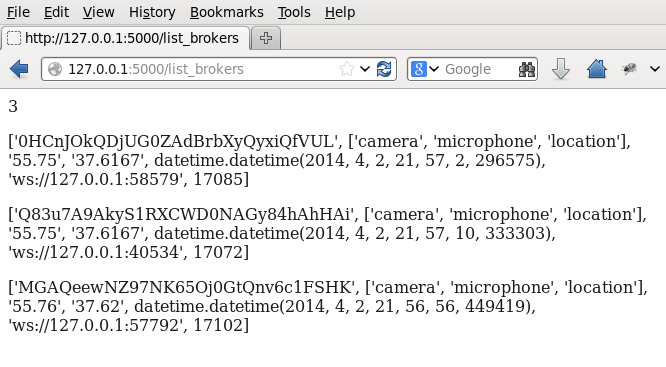
\includegraphics{images/1-clean_producers/small_test_1-1.png}
\caption{Initial list of producers}
\end{figure}

Two of the producers were then killed (by sending SIGINT from the
terminal). After this, the list of producers was still the same, as the
registry only cleans up the producer list either when a consumer
requests data from new producers or when it is explicitly told to (via
the /clean\_producers API call). After this call was made, the list
looked as follows:

\begin{figure}[H]
\centering
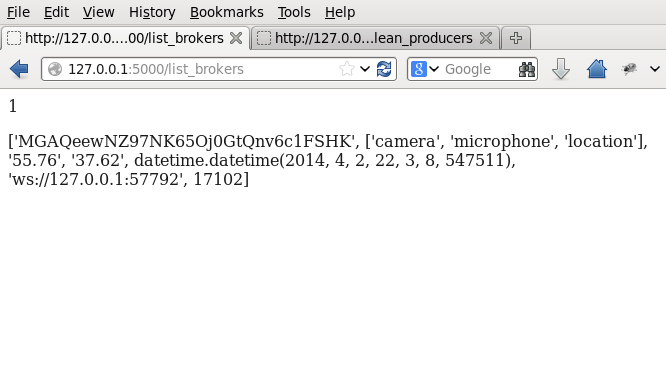
\includegraphics{images/1-clean_producers/small_test_1-3.png}
\caption{Cleaned list of producers}
\end{figure}

When the command is called, the registry prints the ID of any producer
which is being removed to its output stream, which is shown below just
for more confirmation that it actually did happen.

\begin{figure}[H]
\centering
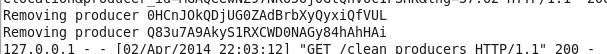
\includegraphics{images/1-clean_producers/small_test_1-4.png}
\caption{Producers which are being removed}
\end{figure}

\subsubsection{Reconnecting With Producers Whose Broker has
Died}\label{reconnecting-with-producers-whose-broker-has-died}

\subsubsection{Rebuilding the Registry After a
Crash}\label{rebuilding-the-registry-after-a-crash}

\section{Reproducing tests}\label{reproducing-tests}

\section{Future work}\label{future-work}

Any system can always be more scalable and robust, and thus there is
much that could be done to improve the system.

There are a few ways the current implementation of the system can be
further improved:

The registry, based on the popular Flask framework, currently can
withstand many hundreds of requests at once. However, at the moment it
is running on the development server (server software, not hardware)
which is not optimised for concurrent requests. Deploying the registry
on a combination of Nginx (high-performance HTTP server) and Gunicorn
(WSGI HTTP server) would allow to ``hide'' multiple registry processes,
responding to the same port. This would considerably improve the
scalability of the registry for concurrent requests. Unfortunately,
deploying Nginx and Gunicorn was problematic on the school's servers.
For now, Flask's development server was used.

With more time, we would have liked to implement distributed brokers
(i.e.~running them on other machines), with the possibility for brokers
to subscribe to and publish data from multiple producers to allow the
system to operate with fewer processes.

\section{Conclusion}\label{conclusion}

A robust message-oriented middleware for mobile sensing was developed.
The system is based on the pub-sub paradigm. It consists of several
components -- producers, consumers, registry, brokers. Components
communicate using modern standards: WebSockets + WAMP and REST.
According to the component specification, a Python implementation was
created, although other languages could easily be used to implement
producers or consumers. The implementation was testing, showcasing good
scalability, robustness, and ability to recover from crashes.
